\documentclass[a4paper,10pt,oneside]{article}
\usepackage[polutonikogreek,italian]{babel}
\usepackage[utf8x]{inputenc}
\usepackage{amsmath}
\usepackage{amsthm}
\usepackage{amssymb}
\usepackage{amscd}
\usepackage[pdftex,colorlinks=true,urlcolor=black]{hyperref}
\usepackage{graphicx}
\usepackage{float}
\usepackage{array}
\usepackage{rotating}
\usepackage[small]{caption}
\usepackage{lscape}
\usepackage{fancybox}
\usepackage{booktabs}
\usepackage[noanswer]{exercise}
\parindent0ex
\renewcommand{\fboxsep}{0.4cm}
\renewcommand{\textfraction}{0.05}
\renewcommand{\topfraction}{0.95}
\renewcommand{\bottomfraction}{0.95}
\renewcommand{\floatpagefraction}{0.35}
\renewcommand{\ExerciseName}{Esercizio}
\renewcommand{\ExerciseListName}{Es}
\setcounter{totalnumber}{5}
\restylefloat{figure}
\begin{document}
\section*{La cinematica}
%\input{immagineIntroduttiva}

\subsection*{Il moto lineare uniforme}
\subsubsection*{Grafici e traiettorie}

La traccia lasciata da un aeroplano trattiene nel tempo la memoria del recente passaggio.\newline
In generale, si definisce {\bfseries traiettoria} l'insieme dei punti dello spazio occupati da un oggetto durante il proprio movimento.\newline
La traiettoria, tuttavia, offre una rappresentazione parziale del movimento. Osservando il solco tracciato su una pista di terra da una bicicletta non è possibile comprendere se il ciclista stesse pedalando lentamente o a ritmo sostenuto. Per una descrizione completa, è necessario acquisire anche informazioni relative agli istanti nei quali l'oggetto in movimento ha occupato ciascuna posizione.
\newline

Una descrizione completa di un moto è una {\bf \slshape funzione dello spazio nel tempo}, nella quale ad ogni singolo istante è associata la posizione occupata dall'oggetto nello spazio.
\newline

Di solito la rappresentazione di un moto è un'attività complessa, perché lo spazio è un'entità tridimensionale e richiede quindi la definizione di una funzione a 3 valori.
Tuttavia, siccome ciascuna posizione può essere scomposta nelle proprie componenti unidimensionali, è utile occuparsi, all'inizio, del cosidetto {\bf \slshape moto lineare}, nel quale la traiettoria del corpo è un {\bf \slshape sottoinsieme} della retta.
\newline

Per rappresentare il moto lineare, è particolarmente efficace riportare la traiettoria sull'asse verticale del piano cartesiano e il tempo su quello orizzontale. I punti di questo piano (che non sono nè punti dello spazio, nè istanti del tempo, proprio perché composti da una coordinata spaziale e da una coordinata temporale) vengono chiamati {\bf eventi}.

Pertanto, l'osservazione di un moto consiste nel rilievo di un certo numero finito di eventi discreti \footnote{spesso, nel linguaggio scientifico, il termine {\slshape discreto} è utilizzato come sinonimo di {\slshape separato} o {\slshape distinto}.}.
Se rappresentiamo gli eventi che descrivono un moto reale su un grafico spazio-tempo, possiamo fare delle osservazioni globali, che permettono di descrivere le caratteristiche del moto nel suo insieme.\newline

Il primo elemento importante da riconoscere è la distanza temporale che separa, a coppie, gli eventi nel tempo, che viene chiamata è chiamata intervallo di tempo ed è indicata spesso dal simbolo $\Delta t$:
\begin{center}
\begin{math}
\Delta t = t_{finale}-t_{iniziale}
\end{math}
\end{center}
Allo stesso modo, è importante verificare se il corpo, durante l'osservazione, ha modificato la propria posizione. Si può definire quindi lo spostamento $\Delta s$ come:
\begin{center}
\begin{math}
\Delta s = s_{finale} - s_{iniziale}
\end{math}
\end{center}
Per ogni coppia di eventi del grafico spazio tempo, si definisce {\bf velocità media} il rapporto tra lo spazio percorso e il tempo impiegato:
\begin{center}
\begin{equation}
v_{media}=\frac {\Delta s}{\Delta t}=\frac {s_{finale} -s_{iniziale}}{t_{finale}-t_{iniziale}}
\end{equation}
\end{center}
La velocità media è una proprietà associata esclusivmente due eventi - evento iniziale ed evento finale - che intervengono nella definizione. Se una automobile percorre dieci chilometri in dieci minuti, non possiamo sostenere che abbia transitato in tutti i punti del proprio percorso alla velocità di $60 \frac {km}{h}$, senza neppure fermarsi ai semafori. Tuttavia, l'osservazione di un campione abbastanza nutrito di eventi, sufficientemente ravvicinati nel tempo, ci induce qualche volta ad avanzare delle ipotesi relative ad eventi per quali non è stata operata una misura reale.
\newline

Supponiamo di rilevare alcuni passaggi di un podista sulla linea di arrivo di una pista di atletica, durante una gara su diecimila metri, e di riportarli su una tabella come la seguente:
\begin{center}
\begin{tabular}{| c | c |}
\hline
giri di pista & intervallo di tempo (s) \\
\hline
7° &  0 \\
\hline
9° & 144 \\
\hline
12° & 360 \\
\hline
16° & 648 \\
\hline
18° & 792 \\
\hline
23° & 1142 \\
\hline
\end{tabular}
\end{center}

In questo esempio, la rilevazione è cominciata al settimo giro di pista, quando il podista aveva già percorso 2800 metri (sette giri, appunto). I successivi rilievi riportano il tempo misurato a partire dal settimo giro. Ecco come può essere rappresentato il moto con geogebra:
\begin{figure}[H]
 \centering
 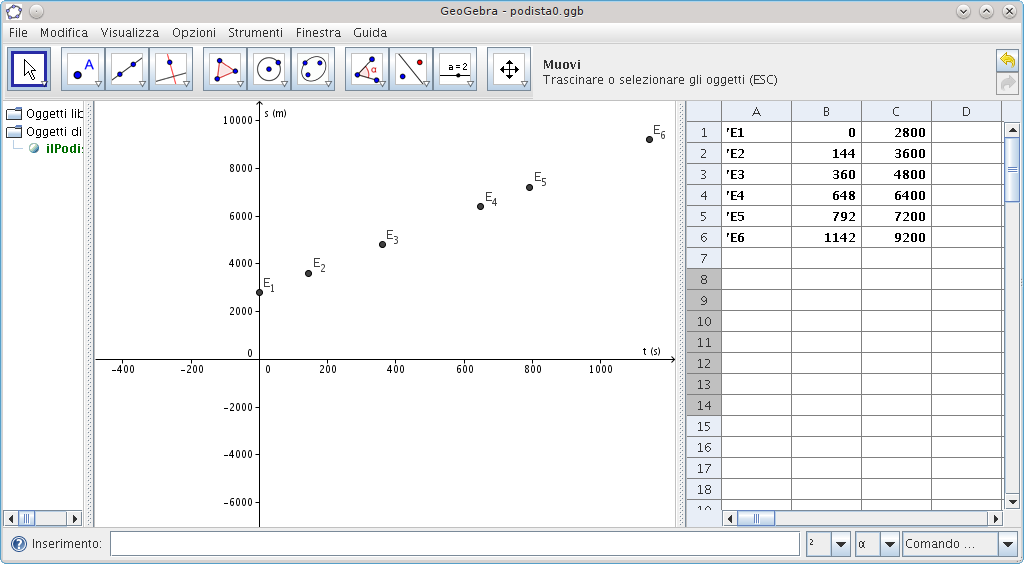
\includegraphics[width=.7\textwidth]{../immagini/podista.png}
 % podista.png
 \label{fig:il grafico spazio tempo di un podista}
\end{figure}

A prima vista, i punti appaiono ben allineati. Valutiamo, per alcune coppie di punti, i valori degli incrementi e delle velocità relative.
\begin{figure}[H]
 \centering
 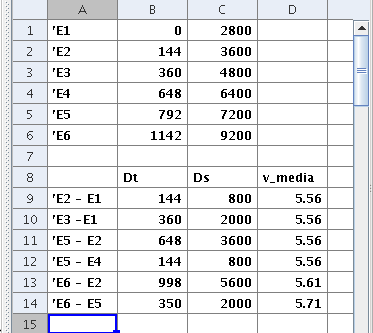
\includegraphics[width=.7\textwidth]{../immagini/podista1.png}
 % podista.png
 \label{fig:il grafico spazio tempo di un podista}
\end{figure}

In questo esempio, sono stati scelti soltanto alcuni dei possibili accoppiamenti tra i sei punti dell'esempio. Possiamo osservare, tuttavia, che la terza colonna, relativa alle velocità medie, contiene valori identici per tutti gli accoppiamenti, tranne che per le coppie di eventi in cui compare l'evento $E_6$, che contiene valori leggermente più alti.\newline
Questi calcoli ci portano a dedurre che il podista possa aver marciato fino al diciottesimo giro ad una velocità costante, e abbia incrementato leggermente il ritmo nei seguenti cinque giri.\newline
A questo punto, potremmo verificare con più attenzione l'allineamento dei punti del grafico, e osserveremmo che l'ultimo si discosta leggermente dalla linea dei precedenti.
\newline

Viene spontaneo, a questo punto, constatare l'analogia tra il concetto di velocità e il concetti di coefficiente angolare usato per descrivere la direzione delle rette nello spazio. In un grafico spazio-tempo, infatti, la velocità media tra due eventi è rappresentata dall'inclinazione del segmento che li unisce.
\newline

Osserviamo ancora i primi cinque punti del grafico. Come già detto, siccome sono tutti perfettamente allineati, ogni coppia di eventi definisce una velocità media uguale a tutte le altre, pari a $5,56 \frac ms$. Il fatto suggerisce l'ipotesi che il podista abbia rispettato la stessa condizione per tutti gli istanti compresi dal settimo al sedicesimo giro. Sulla base di questa assunzione, possiamo realizzare un modello del moto, tracciando una retta che unisca i cinque punti. Per farlo, basta utilizzare l'equazione $(4)$ del capitolo precedente, scrivendo:
\begin{center}
\begin{equation}
\label{eq:Equazione oraria del moto lineare uniforme}
s = s_0 + v (t -t_0)
\end{equation}
\end{center}
Questa equazione si chiama {\bf Equazione oraria del moto lineare uniforme}.\newline
che nel nostro caso diventa:
\begin{center}
\begin{math}
s = 2800 + 5.56 t
\end{math}
\end{center}
Confrontiamo graficamente i dati sperimentali con il modello teorico:
\begin{figure}[H]
 \centering
 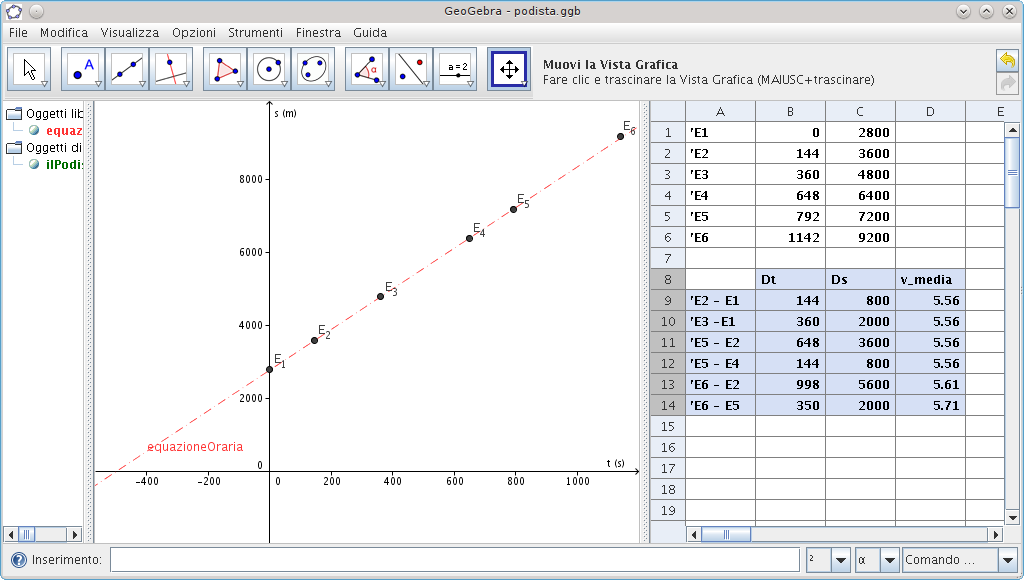
\includegraphics[width=.7\textwidth]{../immagini/podista2.png}
 % podista.png
 \label{fig:confronto dei dati con il modello}
\end{figure}


L'equazione data, ci permette di effettuare operazioni di interpolazione e di estrapolazione. Se ad esempio, ci chiediamo dopo quanto tempo il nostro modello prevede il passaggio del podista al decimo giro, possiamo semplicemente sostituire la posizione 4000 all'equazione oraria e ricavare il tempo $t$ come incognita:
\begin{center}
\begin{math}
t = \frac {s -s_0} {v} = \frac {4000 - 2800} {5.56} = 216 s
\end{math}
\end{center}
Siccome l'evento $(216;4000)$ è compreso all'interno dei cinque punti rilevati, parleremmo in questo caso di interpolazione.\newline
Potremmo invece effettuare delle estrapolazioni se desiderassimo valutare, sulla base del nostro modello, il tempo in cui avremmo atteso il passaggio del podista al ventitreesimo giro o il tempo di partenza della gara:
\begin{center}
\begin{math}
t = \frac {s -s_0} {v} = \frac {9200 - 2800} {5.56} = 1152 s
\end{math}
\end{center}
Il tempo atteso al ventitreesimo giro sarebbe stato 1152 s. Il podista, quindi, è transitato con un anticipo di 10 secondi, rispetto al modello teorico.
\begin{center}
\begin{math}
t = \frac {s -s_0} {v} = \frac {0 - 2800} {5.56} = - 504 s
\end{math}
\end{center}
Il tempo stimato di avvio della gara precede di 504 secondi il passaggio al settimo giro.
\newline

Il modello  che abbiamo utilizzato in questo esempio è un modello di {\bf moto a velocità constante}.
La velocità di uno spostamento è costante se, preso comunque un intervallo di tempo, la velocità media relativa agli estremi di quell'intervallo è sempre la stessa.\newline
Il concetto di velocità costante sottende quello di {\bf velocità istantanea}. Se un moto avviene a velocità constante, infatti, possiamo cosiderare la velocità come una proprietà di ciascun instante del moto, preso singolarmente. In seguito, renderemo più generale questo concetto per applicarlo a moti a velocità variabile.

\subsubsection*{I grafici velocità tempo}

Non sempre la rappresentazione di un moto consiste nella descrizione della posizione nello spazio.\newline
Immaginiamo di condurre un’automobile lungo un autostrada in una notte di
nebbia molto fitta, che rende del tutto impossibile la visione dei cartelli stradali,
costringendo l’autista a marciare lentamente lungo li brdo della corsia. In queste condizioni, l’unico strumento utile, per determinare la posizione del veicolo, è esclusivamente il tachimetro di bordo.\newline
Ora, i tachimetri sono strumenti progettati per misurare la velocit` in un modo diretto, come se fosse una grandezza primitiva, dalla quale, eventualmente,
sarebbe possibile dedurre una misura derivata di spostamento.
\newline

Considerata la difficoltà e la pericolosità intrinseca di una navigazione nella nebbia, l’autitsta dovr` fare attenzione, prima di tutto, a non assumere una velocità troppo elevata, ma neppure una velocit` troppo bassa, per risultare d’intralcio
ad altri veicoli in marcia dietro al proprio. Di conseguenza, bisognerà usare moltissima attenzione a mantenere il contachilometri sempre nella stessa posizione,
realizzando quello che si chiama un moto a velocità costante.\newline

La rappresentazione grafica di un moto derivato da una successione di misure
di velocità si chiama grafico velocità-tempo.\newline
Il grafico velocità-tempo di un moto a velocità costante assomiglia a quello sotto
riportato:
\begin{figure}[H]
 \centering
 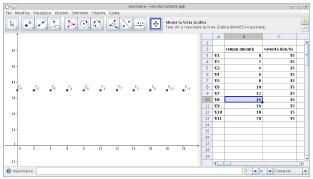
\includegraphics[width=.7\textwidth]{../immagini/velocitaCostante.jpeg}
 % podista.png
 %\label{fig:il grafico velocità tempo di un moto costante}
\end{figure}

Anche in questo caso, dai punti sperimentali è possibile derivare una retta, che risulta rigorosamente parallela all’asse dei tempi. Ma a noi interessa il modo in cui ` possibile ricavare informazione sullo spostamento dell’oggetto in movimento. Siccome, per definizione, la velocità di un moto costante è uguale allo spazio percorso diviso per il tempo impiegato, possiamo dedurre, a rovescio che, conoscendo la velocità e l’intervallo di tempo, si possa ricavare lo spazio da una moltiplicazione:
\begin{center}
\begin{math}
\Delta s = v * \Delta t 
\end{math}
\end{center}

Guardando bene la figura seguente, si può aggiungere anche un’importante osservazione di carattere grafico: il prodotto della velocità per l’intervallo di tempo è uguale all’area di un rettangolo.
\begin{figure}[H]
 \centering
 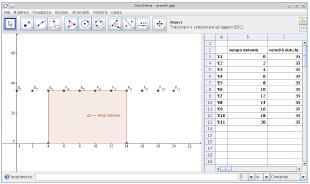
\includegraphics[width=.7\textwidth]{../immagini/spazioSottoIlGrafico_v-t.jpeg}
 % podista.png
 %\label{fig:il grafico velocità tempo di un moto costante}
\end{figure}

Bisogna fare attenzione a valutare correttamente l’informazione ricavabile da un grafico spazio tempo. La quantità definita spazio percorso, infatti, va distinta con attenzione dal concetto di posizione. Bisogna ribadire, infatti, che lo spazio percorso è definito come la differenza tra la posizione finale e la posizione iniziale.

Conoscendo, solo lo spazio percorso, non sarà perciò possibile individuare la posizione finale di un oggetto in movimento.
Alle volte, tuttavia, oltre allo spazio percorso, è possibile conoscere anche la posizione iniziale, e in questi casi risulta:
\begin{center}
\begin{math}
s_{finale} = s_{iniziale} + \Delta s = s_{iniziale} + v \Delta t
\end{math}
\end{center}

\subsubsection*{La velocità istantanea}

Fino ad ora, abbiamo quasi utilizzato sempre il concetto di {\slshape velocità` media}, intesa come proprietà associata a una {\slshape coppia} di eventi.\newline
Tuttavia, a volte serve pensare alla velocità come proprietà dello stato di moto di un singolo evento e si parla, in questo caso, di {\bf velocità istantanea}.\newline

Il concetto di velocità istantanea diventa realmente utile quando si studia un moto vario, dove la velocità cambia istante per istante. Quando cioè è possibile ritenere che due istanti diversi, per quanto ravvicinati nel tempo, possano avere
delle velocità diverse.\newline

L’uso del concetto di velocità istantanea, però, non è del tutto immediato e richiede un po’ di riflessione.
La velocità si misura dividendo uno spostamento per un intervallo temporale. Un singolo istante, invece, è un punto nel tempo, che non corrisponde ad alcun intervallo e a cui si può` associare una sola posizione.\newline

Pensiamo a un ciclista che transita sul traguardo alla velocità di 50 chilometri orari. Avrebbe senso domandare: {\slshape Quanto spazio percorre il ciclista nel preciso istante in cui tocca il traguardo?} Chiaramente no. Il transito, infatti, avviene
ad una determinata velocità ma, immediatamente dopo, l’atleta rilascia i pedali e comicia a rallentare. Se volessimo capire quanto spazio dopo il traguardo sia stato percorso in venti secondi, non saremmo in grado di esprimere nessuna previsione. Se però ci limitiamo a ragionare per intervalli di tempo più brevi, ci accorgiamo di poter avanzare delle stime meno grossolane. Proviamo a chiederci, ad esempio, quanto spazio viene percorso dal ciclista nel primo secondo.
Trattandosi di un tempo molto breve, potremmo supporrre che la bicicletta abbia rallentato pochissimo, e potremmo avanzare l’ipotesi di osservare, sia pure per un solo secondo, un moto a velocità costante. Cinquanta chilometri all’ora corrisponde a circa undici metri al secondo. Dunque potremmo immaginare che il ciclista si trovi, dopo un secondo, a circa undici metri dietro al traguardo.\newline

Se ripetiamo lo stesso ragionamento per tempi ancora più brevi, otterremmo risultati ancora più convincenti, cioè affetti da un errore più piccolo. In generale, dire che un oggetto possiede una certa velocità istantanea, significa affermare che considerando un intervallo di tempo abbastanza piccolo, si può valutare lo spazio percorso dalla moltiplicazione della velocità data per l’intervallo di tempo, con errore trascurabile, come se stessimo ossservando un moto a velocità costante.

Proviamo ora ad applicare questa idea a un problema più complesso. Immaginiamo che il ciclista precedente si fermi, dopo l’arrivo, in trenta secondi, frenando in modo uniforme.

Per rappresentare graficamente il movimento, possiamo considerare la figura seguente:

\begin{figure}[H]
 \centering
 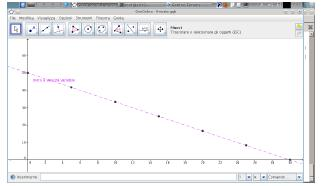
\includegraphics[width=.7\textwidth]{../immagini/frenataUniforme.jpeg}
 % podista.png
 %\label{fig:il grafico velocità tempo di un moto costante}
\end{figure}

Questa curva ci mostra che stiamo osservando un movimento a velocità sempre più lento. Ovvero, un movimento nel quale, a parità di intervallo di tempo, vengono coperti spazi sempre più brevi. Per rappresentare graficamente questa idea, conviene tracciare, intorno alla retta obliqua che rappresenta il moto, una linea spezzata, {\slshape costante a tratti}, come quella nella figura successiva:

\begin{figure}[H]
 \centering
 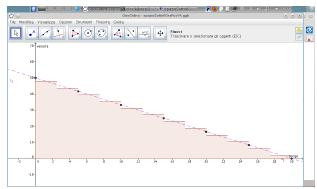
\includegraphics[width=.7\textwidth]{../immagini/scaletta.jpeg}
 % podista.png
 %\label{fig:il grafico velocità tempo di un moto costante}
\end{figure}

In questa immagine, la curva spezzata è un’{\slshape approssimazione} del moto reale. Un’approssimazione è un modello diverso da quello reale, ma costruito con una tecnica tale da avvicinarsi alla realtà con la precisione desiderata. Nell’esempio, il moto è stato suddiviso in dodici intervalli, ma se la suddivisione fosse stata più raffinata, si sarebbe ottenuta una spezzata ancora più simile alla curva originale.\newline
Se osserviamo i singoli rettangoli colorati, sotto ad ogni tratto orizzontale, possiamo osservare che l’area di ciascuno di essi possiede il significato cinematico di spazio percorso. Sapendo che la nostra osservazione è cominciata esattamente nell’istante in cui il ciclista transitava sotto il traguardo, possiamo ricavare dalla curva v-t la posizione esatta del ciclista in ogni istante del proprio moto.\newline

Possiamo cioè dedurre la curva spazio-tempo del moto, che assume l’aspetto di una parabola, come nell’immagine sotto:

\begin{figure}[H]
 \centering
 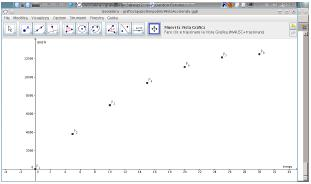
\includegraphics[width=.7\textwidth]{../immagini/curvaSpazioTempo.jpeg}
 % podista.png
 %\label{fig:il grafico velocità tempo di un moto costante}
\end{figure}


L'ordinata di ciscun evento in questa immagine è determinato sommando le aree in rosa della curva velocità tempo. Per esprimere i dati in metri, inoltre, è stato necessario convertire le velocità da chilometri all’ora a metri al secondo.
Nell’immagine si osserva immediatamente che i punti non sono più disposti lungo una linea retta, ma che gli incrementi tra due valori equispaziati nel tempo diminuiscono progressivamente. Questo accade proprio perché la curva velocità tempo osservata dalla quale è stato derivato il grafico è decrescente.\newline

Naturalmente, questa osservazione può essere utilizzata per ragionare nella direzione inversa.\newline
Immaginiamo di produrre una curva sperimentale spazio-tempo di un moto e di voler ricavare da essa un grafico velocità tempo. In questo caso, saremmo interessati a rilevare, per ogni coppia di eventi, il valore della velocità media che, graficamente, è rappresentato dall’inclinazione della retta li congiunge. Questa velocità media sarà un valore diverso per ogni scelta della coppia di punti.
Tuttavia, se osserviamo un insieme di coppie sufficientemente ravvicinate nel tempo, ci viene spontaneo assumere che i valori calcolati delle velocità medie manifestino piccoli cambiamenti, intorno a un determinato valore di riferimento.
Pensandoci ancora meglio, ci possiamo accorgere che questo valore si avvicina al coefficiente angolare della retta tangente alla curva negli estremi dell’intervallo considerato. Questo accade se l’intervallo di tempo tra gli eventi è sufficentemente piccolo da poter essere considerato come un unico istante. Il valore corrispondente della velocità, in questo caso, assume il nome di {\bf velocità istantanea}\footnote {a rigore, questa operazione andrebbe descritta da un processo di limite, ma qui usiamo una descrizione semplificata di tipo qualitativo. seguirà immagine ...}.


\end{document}
